\documentclass[class=report, crop=false]{standalone}
\usepackage{../preamble}

\begin{document}
	% Specific lengths in this document
	\import{../}{default_lengths.tex}
	%
	\chapter{Ứng dụng của cặp ghép và mã hóa dựa~trên định danh}\label{chap:6}
	\section{Ứng dụng lý thuyết}
		\subsection{Lược đồ mật mã xây dựng từ cặp ghép}
			Theo báo cáo của Viện Quốc gia về Tiêu chuẩn và Công nghệ Hoa Kỳ (NIST) về mật mã dựa trên cặp ghép vào năm 2015 \cite{nist_report}, những lược đồ mật mã sau đây đã được xây dựng từ cặp ghép song tuyến tính:
			\vspace{-0.5\baselineskip}
			\begin{itemize}
				\item \textbf{Mã hóa dựa trên định danh (identity-based encryption - IBE)}.
				\item \textbf{Chữ ký dựa trên định danh (identity-based signature - IBS)}.
				\item \textbf{Signcryption}: Lược đồ kết hợp chức năng của mã hóa và chữ ký.
				\item \textbf{Mã hóa dựa trên thuộc tính (attribute-based encryption - ABE)}: Mở rộng của IBE, trong đó người dùng chỉ giải mã được nếu sở hữu tập thuộc tính (tuổi, nghề nghiệp, v.v) khớp với bản mã.
				\item \textbf{Mã hóa tìm kiếm được (searchable encryption)}: Cho phép kiểm tra một từ khóa có hiện diện trong bản mã không mà không biết được bất cứ thông tin gì về từ khóa.
				\item \textbf{Chữ ký ngưỡng (threshold signature)}: Yêu cầu phải có ít nhất $t$ người ký mới tạo ra được một chữ ký hợp lệ.
				\item \textbf{Chữ ký tổng hợp (aggregated signature)}: Từ nhiều chữ ký có thể tạo được một chữ ký tổng hợp ngắn thay thế cho tất cả chữ ký.
				\item \textbf{Chữ ký mù (blind signature)}: Người ký không biết được bất kỳ thông tin gì về văn bản được ký.
				\item \textbf{Chữ ký vòng (ring signature)}: Cho phép bất cứ người nào trong một nhóm cũng có thể ký một chữ ký mà có thể xác nhận là một người nào đó trong nhóm đã ký nhưng không lộ ra là ai.
				\item \textbf{Chữ ký nhóm (group signature)}: Tương tự như chữ ký vòng nhưng có thêm một người quản lý nhóm có thể xác định ai là người đã ký.
			\end{itemize}

			Hơn hết thảy, từ cặp ghép \emph{đa tuyến tính} Garg và các cộng sự \cite{DBLP:conf/focs/GargGH0SW13} đã xây dựng được một mật mã nguyên thủy gọi là \textit{rối hóa bất khả phân biệt} (indistinguishability obfuscation - IO). Đây là một mật mã nguyên thủy cao cấp và có ý nghĩa lý thuyết và ứng dụng rất to lớn. Không ngoa khi nói rằng IO có sức mạnh ngang ngửa với \textit{mã hóa đồng cấu đầy đủ} (fully homomorphic encryption) - mật mã nguyên thủy đang được xem là ``chén thánh'' của mật mã. Tuy nhiên nghiên cứu IO vẫn còn rất sơ khởi và ít người tham gia, vì vậy chưa có nhiều kết quả như mã hóa đồng cấu.
			
			Rối hóa phần mềm là một ý tưởng đã được quan tâm từ lâu, với mục đích là để ngăn chặn \textit{nghiên cứu đảo ngược} (reverse engineering) phần mềm. Kỹ thuật này làm rối mã nguồn và / hoặc mã sau biên dịch của chương trình để người không thể đọc được nhưng vẫn cho phép chương trình chạy đúng. Không ít giải pháp rối hóa đã được xây dựng bởi các tổ chức phần mềm, tuy nhiên không nào trong số đó có thể ngăn chặn được hacker. Đến khi IO được đề xuất như là một sự hình thức hóa khái niệm rối hóa chương trình \cite{DBLP:conf/crypto/BarakGIRSVY01}, cộng với việc xây dựng đầu tiên ra đời vào năm 2013 \cite{DBLP:conf/focs/GargGH0SW13}, chúng ta mới có thể nghĩ đến thế giới mà phần mềm là \emph{không thể bị hack}.
		%
		\subsection{Lược đồ mật mã xây dựng từ hệ IBE}
			Nhờ khả năng tùy biến cao trong việc thiết kế và sử dụng định danh, IBE đã thể hiện tiềm năng lớn trong việc xây dựng các lược đồ mật mã khác từ nó. Những xây dựng này tùy trường hợp có thể cần sự kết hợp với một vài lược đồ nữa. Có thể nói rằng, mỗi khi mật mã được tái xây dựng trên một nền tảng toán học mới, mã hóa dựa trên định danh là một trong những lược đồ cao cấp đầu tiên được tiếp cận sau khi đã có đủ các lược đồ cơ bản.
			%
			\vspace{-\baselineskip}
			\subsubsection{Chữ ký (mặc định)}
				\vspace{-0.5\baselineskip}
				Nếu xây dựng được một hệ IBE thì mặc nhiên ta được tặng kèm miễn phí thêm một hệ chữ ký. Xem khóa bí mật chủ và khóa công khai chủ trong hệ IBE tương ứng là khóa bí mật và khóa kiểm tra trong hệ chữ ký. Lúc này thuật toán sinh khóa là thuật toán ký và thuật toán mã hóa kết hợp giải mã là thuật toán kiểm tra chữ ký. Cụ thể, để ký một văn bản $M$ thì ta xem $M$ như định danh trong hệ IBE rồi tạo chữ ký là khóa bí mật cho ``định danh'' $M$. Sau khi nhận được chữ ký, thuật toán kiểm tra chọn ngẫu nhiên một bản rõ của hệ IBE, sau đó mã hóa trên định danh $M$ rồi lại giải mã bằng chữ ký. Nếu bản rõ sau khi giải khớp với ban đầu thì chữ ký hợp lệ. Tính~không giả mạo được của chữ ký tương đương với việc mọi thực thể khác PKG đều không thể sinh khóa bí mật của định danh. Ở đây thuật toán kiểm tra là ngẫu nhiên, nhưng với một hệ IBE được cho cụ thể, ta có thể chỉnh sửa để được thuật toán kiểm tra đơn dịnh. Ví dụ như thuật toán \textsf{SecretKeyVerify} của hệ mã BBG trước đó.
			%
			\vspace{-\baselineskip}
			\subsubsection{Mã hóa khóa công khai an toàn IND-CCA}
				\vspace{-0.5\baselineskip}
				Như đã nói ở mục \ref{chap:2.related_works}, biến đổi CHK hoặc biến đổi BK có thể được áp dụng lên một hệ IBE an toàn IND-sID-CPA bất kỳ. Kết quả thu được là một hệ mã hóa khóa công khai an toàn IND-CCA. Trong hệ này khóa bí mật chủ và khóa công khai chủ tương ứng đóng vai trò của khóa bí mật và khóa công khai.
			%
			\vspace{-\baselineskip}
			\subsubsection{Mã hóa khóa công khai hỗ trợ tìm kiếm từ khóa (public-key encryption with keyword search - PEKS)}
				\vspace{-0.5\baselineskip}
				Lược đồ này được đề xuất bởi Boneh và các cộng sự \cite{DBLP:conf/eurocrypt/BonehCOP04}, thuộc vào nhóm hệ mã hóa tìm kiếm được. Một hệ PEKS bao gồm bốn thuật toán \textsf{KeyGen, Trapdoor, PEKS,~Test}. Đầu tiên một cặp khóa công khai/bí mật $(pk, sk)$ được sinh bởi thuật toán \textsf{KeyGen}. Thuật toán \textsf{PEKS} từ $pk$ và một từ khóa $W$ tạo ra một bản mã tìm kiếm được của $W$, gọi là $S_W$. Mặt khác, thuật toán \textsf{Trapdoor} nhận tham số là $sk$ cùng với một từ khóa $W'$ và tạo ra một cửa lật (trapdoor) $T_{W'}$ để kiểm tra từ khóa. Cuối cùng thuật toán \textsf{Test} nhận vào $(pk, S_W, T_{W'})$ và kiểm tra xem $W$ có bằng $W'$.
				%
				\newpage
				Ta thấy rằng hệ PEKS rất tương đồng với hệ IBE, với từ khóa đóng vai trò định danh, thuật toán \textsf{Trapdoor, PEKS, Test} tương ứng với thuật toán \textsf{SecretKeyGen, Encrypt, Decrypt}. Một điểm khác là hệ PEKS không phải mã hóa nên thuật toán \textsf{PEKS} không nhận vào bản rõ và \textsf{Test} trả về kết quả kiểm tra thay vì bản rõ. Vì sự tương đồng này, nhiều hệ PEKS đã lấy ý tưởng từ những hệ IBE sẵn có. Một tiêu chí an toàn của PEKS là yêu cầu bản mã tìm kiếm được $S_W$ không để lộ bất cứ thông tin gì về $W$ trừ khi có $T_W$. Điều này là để phục vụ cho \textit{truy xuất thông tin riêng tư} (private information retrieval). Vì lý do này việc xây dựng PEKS thường xuyên xuất phát từ những hệ IBE có tính ẩn danh.
			
				Trong phạm vi hiểu biết của mình, sinh viên vẫn chưa biết phép biến đổi tổng quát nào biến một hệ IBE bất kỳ thành một hệ PEKS. Tuy nhiên chiều ngược lại là có. Cũng trong \cite{DBLP:conf/eurocrypt/BonehCOP04}, các tác giả đã chỉ ra rằng chỉ bằng một số chỉnh sửa nhỏ trên một hệ PEKS là ta có ngay một hệ IBE.
			%
			\vspace{-\baselineskip}
			\subsubsection{Mã hóa an toàn trong tương lai}
				\vspace{-0.5\baselineskip}
				Một hệ \textit{mã hóa khóa công khai an toàn trong tương lai} (forward-secure public key encryption - fsPKE) cho phép những bản mã được tạo ra ở một thời điểm nào đó trong quá khứ không bị mất an toàn trong trường hợp khóa bí mật ở tương lai bị lộ hoặc suy~yếu. Hệ mã này trong pha thiết lập phải chỉ định một số $N$ là số khoảng thời gian của hệ mã. Khoảng thời gian đếm từ 0 đến $N - 1$ xem như từ lúc thiết lập hệ đến tương lai. Khóa bí mật của khoảng thời gian thứ $i$ không thể được dùng để giải những bản mã được mã hóa bằng khóa công khai của khoảng thời gian từ $0$ đến $i - 1$. Để đạt được điều này hệ mã có thuật toán cho phép cập nhật khóa bí mật mỗi khi qua khoảng thời gian mới. Khóa công khai tùy hệ mã có thể cần cập nhật hoặc không.

				Canetti, Halevi và Katz \cite{DBLP:conf/eurocrypt/CanettiHK03} đã xây dựng được một bộ khung hiệu quả từ một hệ \textit{mã hóa cây nhị phân} (binary tree encryption - BTE) bất kỳ có chiều cao cây $\ell$, tạo ra một hệ fsPKE có số khoảng thời gian $N$ bằng số nốt trên cây là $2\,^{\ell + 1} - 1$. BTE bản chất là hệ HIBE với ràng buộc định danh nguyên thủy chỉ thuộc $\{0, 1 \}$. Khóa bí mật của khoảng thời gian $i$ có thể giải mã được tất cả bản mã thuộc khoảng thời gian từ $i$ đến $N - 1$, nhưng không thể với bản mã thuộc khoảng thời gian từ $0$ đến $i - 1$.
				%
				\newpage
				Kích thước khóa bí mật của hệ fsPKE kết quả là $\mathcal{O}(\ell \cdot \delta)$ với $\delta$ là kích thước khóa bí mật định danh của hệ BTE. Khóa công khai cũng chính là khóa công khai chủ của hệ BTE. Sử dụng bộ khung CHK với hệ mã BBG, ta thu được một hệ fsPKE có kích thước khóa công khai, khóa bí mật và bản mã tại mọi thời điểm lần lượt là $\mathcal{O}(\ell)$, $\mathcal{O}(\ell\,^c)$ và $\mathcal{O}(1)$ (với $c$ là hằng số nào đó).

				Ngoài ra, bằng cách cho mỗi người dùng tự áp dụng bộ khung CHK lên chính mình, xem khóa bí mật định danh là khóa của khoảng thời gian $0$, từ một hệ HIBE không giới hạn số cấp sinh khóa (xem lại mục nhỏ \ref{chap2:sec4:restrict_key_derivation}) ta có thể xây dựng được một hệ HIBE an toàn trong tương lai.
	%
	\section{Ứng dụng thực tiễn}
		\subsection{Email}
			Gửi email mã hóa là ứng dụng đơn giản nhất của mã hóa dựa trên định danh, bằng cách dùng email làm định danh. Ứng dụng này có thể được mở rộng bằng cách cho một nhóm người chia sẻ chung một định danh và khóa bí mật. Khi đó ta có thể gửi tin phát tán cho nhiều người chỉ với một bản mã.

			Một ví dụ cụ thể, giả sử Ban giám hiệu Trường Đại học Khoa học Tự nhiên muốn triển khai hệ thống email cho cán bộ, giảng viên. Hệ thống này cho phép mỗi cán bộ được đọc tất cả email gửi cho khoa/bộ môn mình thuộc về nhưng không được đọc email của khoa/bộ môn khác. Khi đó trường chỉ cần xây dựng một hệ HIBE có số cấp tối đa là 3 với định danh cấp 1, 2 và 3 lần lượt là tên khoa, tên bộ môn và tên cán bộ, kết hợp với việc ràng buộc mọi email được gửi tới trường phải tuân thủ nguyên tắc dùng định danh. Ban giám hiệu là PKG có thể kiểm soát được mọi thông tin nội~bộ. Ban chủ nhiệm mỗi khoa sẽ được cấp khóa bí mật cấp 1 của khoa mình. Ví dụ Ban chủ nhiệm Khoa Công nghệ thông tin sẽ được cấp khóa của định danh ``Khoa Công nghệ thông tin''. Mỗi trưởng bộ môn sẽ được cấp khóa bí mật cấp 2 của định danh có dạng (<Khoa>, <Bộ môn>). Ví dụ Trưởng Bộ môn Công nghệ tri thức, Khoa Công nghệ thông tin sẽ được cấp khóa bí mật cho định danh (``Khoa Công nghệ thông tin'', ``Bộ môn Công nghệ tri thức''). Cuối cùng, mỗi cán bộ sẽ được cấp bốn khóa bí mật trên định danh có dạng lần lượt là:
			%
			\begin{itemize}[itemindent=1cm]
				\item[] ``ALL'',
				\item[] (<Khoa>, ``ALL''),
				\item[] (<Khoa>, <Bộ môn>, ``ALL''),
				\item[] (<Khoa>, <Bộ môn>, <Tên cán bộ>).
			\end{itemize}
			
			Ba định danh đầu có thể được xem như là hộp thư chung của toàn trường, khoa và bộ môn. Định danh thứ tư là hộp thư cá nhân.
			%
			\begin{figure}[h] 
				\captionsetup{font=normalsize}
				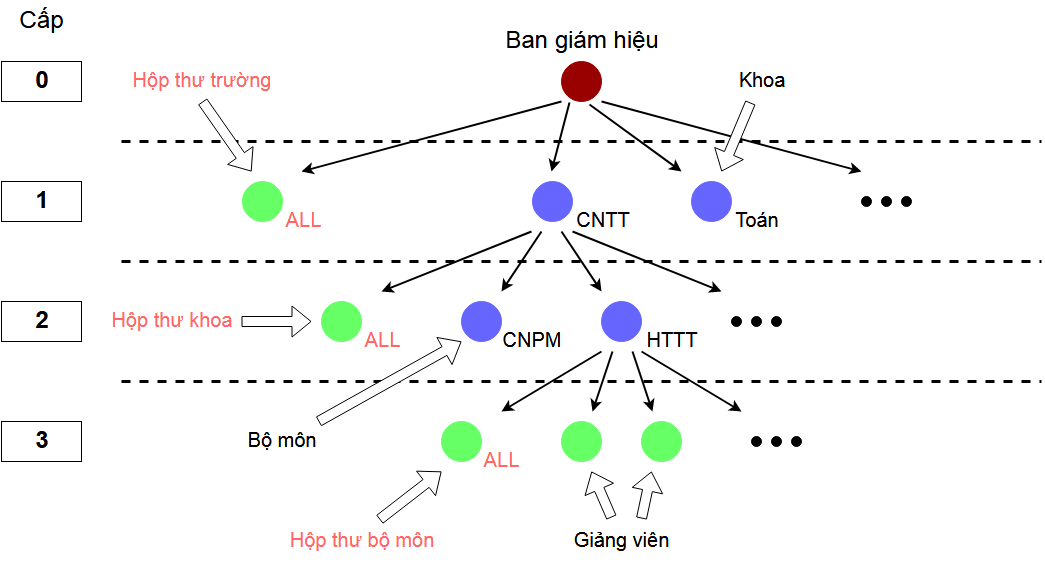
\includegraphics[width=\textwidth]{application_email.png}
				\centering
				\caption{Ứng dụng IBE vào email}
			\end{figure}

			Ứng dụng vào quản lý nội bộ tổ chức là cực kỳ phù hợp với (H)IBE do bởi tính giám hộ khóa vốn có. Tuy nhiên một vấn đề khác phát sinh là không ai kể cả PKG có thể kiểm soát được việc chia sẻ khóa bí mật định danh. Ngay sau khi PKG cấp khóa cho một định danh thì người nhận khóa đã có thể rò rỉ trái phép khóa đó cho những người khác vốn không thuộc nhóm chia sẻ định danh. Giải quyết vấn đề này cần sử dụng những kỹ thuật của \textit{truy vết phản bội} (traitor tracing). Độc giả có thể tham khảo ở \cite{DBLP:conf/pkc/AbdallaDMNPS07}.
		%
		\subsection{Sao lưu tự động an toàn}
			Xét ví dụ sau, một ứng dụng phần mềm có một server A vận hành ứng dụng và một server B thực hiện sao lưu dữ liệu từ server A theo chu kỳ ngày. Người quản trị triển khai cơ chế mã hóa công khai. Khi sao lưu, A mã hóa dữ liệu bằng khóa công khai rồi gửi B. Bằng khóa riêng tư được người quản trị cài đặt cho, B giải mã rồi lưu vào cơ sở dữ liệu. Trong trường hợp một người tấn công nào đó biết được khóa riêng tư và bắt được tất cả dữ liệu giao tiếp của A và B, hắn sẽ biết toàn bộ dữ liệu.
			
			Để phòng ngừa khả năng này, người quản trị thay vào đó có thể triển khai một hệ IBE và cài đặt A mã hóa dữ liệu theo định danh là ngày hiện thời. Ở phía B, người quản trị chỉ cài vào một lượng nhỏ khóa bí mật để giải mã (chẳng hạn số khóa cho một tuần). Người quản trị giữ khóa bí mật chủ và theo chu kỳ cung cấp thêm khóa bí mật định danh cho B. Bằng phương pháp này thiệt hại được giảm xuống đáng kể.
			%
			\begin{figure}[h] 
				\captionsetup{font=normalsize}
				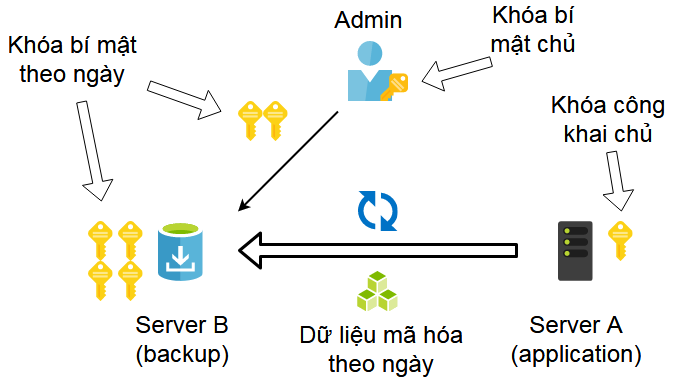
\includegraphics[width=0.7\textwidth]{application_backup.png}
				\centering
				\caption{Ứng dụng IBE vào sao lưu dữ liệu}
			\end{figure}

			Một kỹ thuật để giảm chi phí quản lý của người quản trị là áp dụng hệ mã hóa an toàn trong tương lai nói trên. Khi đó B có thể tự cập nhật khóa và người quản trị không còn cần cấp khóa mới cho B. Tuy nhiên cần chú ý là với bộ khung CHK thì khi khóa của B bị lộ mọi dữ liệu truyền về sau sẽ bị mất an toàn. Vì vậy người quản trị cần có cách phát hiện khi khóa bị lộ để dừng sử dụng khóa và thiết lập lại hệ thống.
		%
		\subsection{Giao tiếp hoàn toàn ẩn danh}
			Với một hệ IBE có tính ẩn danh, ta có thể xây dựng một hệ thống giao tiếp có tính ẩn danh cao và tin cậy. Ví dụ, người quản trị hệ thống triển khai hệ IBE ẩn danh và cấp khóa cho tất cả người dùng. Giả sử Alice và Bob là hai người dùng và Alice muốn gửi tin cho Bob. Khi đó Alice mã hóa thông điệp bằng định danh của Bob và gửi cho tất cả người dùng trong hệ thống. Mỗi người dùng sẽ thử giải mã để biết có phải thông điệp được gửi cho mình không. Và tất nhiên không ai ngoài Bob có thể giải mã được. Nhớ rằng bản mã trong hệ IBE không mang bất cứ thông tin nào của Alice, và với tính ẩn danh của hệ thì bản mã cũng không làm lộ ra Bob là người nhận.
			%
			\begin{figure}[h] 
				\captionsetup{font=normalsize}
				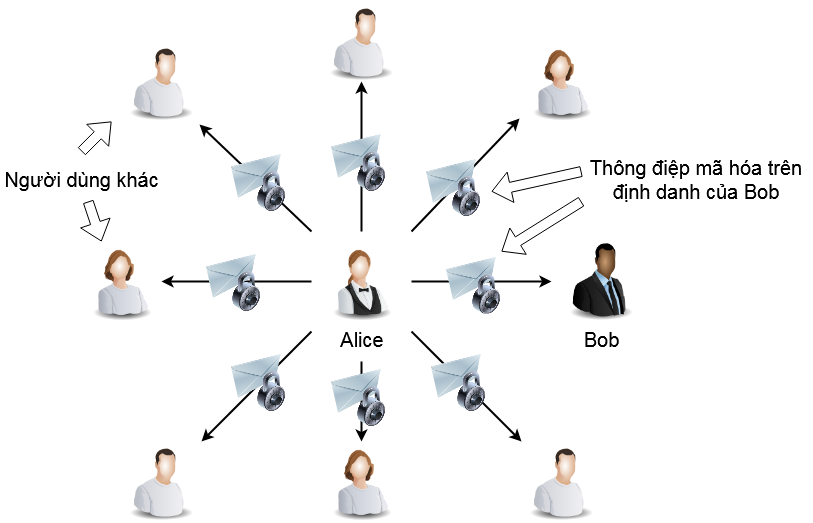
\includegraphics[width=\textwidth]{application_anonimous.png}
				\centering
				\caption{Ứng dụng IBE vào giao tiếp ẩn danh}
			\end{figure}
			
			Thêm vào đó, khác với PKI là khi mỗi lần Alice muốn gửi tin cho Bob, Alice phải truy vấn CA về tình trạng khóa của Bob, dẫn đến lộ thông tin là hai người có giao tiếp với nhau; trong IBE thì Alice không cần bất cứ liên lạc nào với bên ngoài để biết tình trạng khóa của Bob, bằng cách áp dụng kỹ thuật đã trình bày ở mục \ref{chap2:sec5:key_revocation}. Kết hợp với việc Alice gửi tin phát tán đến tất cả người dùng, thiết kế hệ thống này hoàn toàn chống được \textit{tấn công phân tích đường truyền} (traffic analysis attack).

			Một chi tiết kỹ thuật cần nói thêm, trong những hệ IBE ẩn danh thì kể cả chủ sở hữu khóa bí mật để giải cũng không có cách nào kiểm tra một bản mã có phải được gửi đến mình không, ngoại trừ việc giải mã và xem bản rõ thu được có ``bình thường'' không (chẳng hạn như bản rõ phải là ngôn ngữ tự nhiên). Nhưng với không gian bản rõ là các chuỗi ký tự lạ (ví dụ như dữ liệu tiền mã (cryptocurrency)), việc kiểm tra như trên là không thể. Dù vậy ta vẫn có thể giải quyết vấn đề này bằng cách ràng buộc định dạng hoặc áp dụng padding cho bản rõ trước khi mã hóa. Đơn giản nhất ta có thể nối thêm $n$ số 0 vào cuối bản rõ. Với $n$ càng lớn thì xác suất có một quá trình giải mã thất bại mà lại xuất ra bản rõ kết quả có $n$ số 0 ở sau càng thấp.
		%
		\subsection{Mã hóa tìm kiếm được}
			Như đã nói, IBE liên quan mật thiết với PEKS. Giả sử như Alice muốn ủy quyền cho email server phân loại những email đã mã hóa được gửi đến mình, và cô ấy muốn phân loại email theo các từ khóa ``khẩn cấp'', ''công việc'', ``hẹn hò'', v.v. Khi đó cô ấy cần sinh khóa và tạo ra các cửa lật kiểm tra cho các từ này, sau đó gửi cho email server để ủy quyền phân loại. Những người gửi email cho Alice cần phải đính nhãn là bản mã của từ khóa họ muốn kèm theo email. Do đó để hệ thống hoạt động được cần có sự thống nhất từ khóa giữa hai bên và quan trọng là sự hợp tác của người gửi.

			Với một hệ PEKS tương ứng với một hệ HIBE ẩn danh, ta có thể sáng tạo nhiều thiết kế thú vị. Xét một hệ PEKS tương ứng hệ HIBE ẩn danh có số cấp tối đa 2. Nếu~thiết lập định danh (nguyên thủy) cấp 1 là định danh của người nhận và định danh cấp 2 là từ khóa, ta nhận được một hệ \textit{mã hóa dựa trên định danh hỗ trợ tìm kiếm từ khóa} (identity-based encryption with keyword search - IBEKS). Khi đó mọi người dùng trong hệ thống đều có thể ủy quyền tìm kiếm từ khóa trên định danh của mình, không cần một chủ thể trung tâm đóng vai trò này. Với số cấp tối đa lớn hơn ta có thể thiết kế tìm kiếm mịn hơn.

			Ngoài bối cảnh truyền nhận tin, PEKS còn rất hữu hiệu trong việc xây dựng nhật ký giám sát (audit log) mã hóa và tìm kiếm được \cite{DBLP:conf/ndss/WatersBDS04}.
	%
	\newpage
	\section{Những tiêu chuẩn về IBE}
		Dù nghiên cứu mật mã lý thuyết tiến xa tới đâu, cũng không được phép sử dụng trong thế giới thực nếu không có các tiêu chuẩn được công bố bởi các tổ chức tiêu chuẩn quốc tế. Những tổ chức quản lý tiêu chuẩn lớn trong giới mật mã gồm có NIST, IEEE, IETF và ISO. Sau đây sinh viên xin liệt kê một số tiêu chuẩn và văn bản RFC (Request For Comments) liên quan đến IBE và cặp ghép:
		%
		\vspace{-0.5\baselineskip}
		\begin{itemize}[leftmargin=1cm]
			\item \textbf{IEEE P1363.3-2013}: IEEE Standard for Identity-Based Cryptographic Techniques using Pairings
			\item \textbf{ISO/IEC 15946}: Cryptographic techniques based on elliptic curves
			\item \textbf{IETF RFC 5091}: Identity-Based Cryptography Standard (IBCS) \#1: Supersingular Curve Implementations of the BF and BB1 Cryptosystems
			\item \textbf{IETF RFC 5408}: Identity-Based Encryption Architecture and Supporting Data Structures
			\item \textbf{IETF RFC 5409}: Using the Boneh-Franklin and Boneh-Boyen Identity-Based Encryption Algorithms with the Cryptographic Message Syntax (CMS)
			\item \textbf{IETF RFC 6508}: Sakai-Kasahara Key Encryption (SAKKE)
			\item \textbf{IETF RFC 6509}: MIKEY-SAKKE: Sakai-Kasahara Key Encryption in Multimedia Internet KEYing (MIKEY)
		\end{itemize}
		
		Trong số trên chỉ có IEEE P1363.3-2013 và ISO/IEC 15946 là tiêu chuẩn áp dụng được cho Internet và công nghiệp. RFC là những văn bản thông tin mang tính tham khảo được cộng đồng gửi lên IETF và cũng nhờ cộng đồng xét duyệt. Cho đến năm 2015 NIST vẫn chưa đưa ra bất kỳ tiêu chuẩn nào về mật mã dựa trên định danh. Sinh~viên chưa tìm được thông tin về thời điểm hiện tại.

		Tiến trình phát triển tiêu chuẩn cho IBE chậm và chỉ có các hệ mã đời đầu cho thấy nhu cầu sử dụng ngoài thực tế không quá lớn, mặc dù IBE đã đạt độ chín và ý nghĩa nó đem lại là không hề nhỏ.
	\newpage
	%
	% Reset default lengths
	\import{../}{default_lengths.tex}
\end{document}
